\documentclass[10pt, compress]{beamer}

\usetheme[usetitleprogressbar]{m}

\usepackage{booktabs}
\usepackage{amsmath}
\usepackage{nicefrac}
\usepackage{color}
\usepackage{wrapfig}

\newcommand\DP{\delta p}
\newcommand\dd{\mathrm{d}}
\newcommand\ul{\underline}
\newcommand\uul[1]{\underline{\underline{#1}}}
\newcommand\ult[1]{\tilde{\underline{#1}}}
\newcommand\uult[1]{\tilde{\underline{\underline{#1}}}}

\newcommand\matlab{MATLab\textsuperscript{\textregistered}}
\renewcommand\equiv{\Leftrightarrow}
\newcommand\diag{\mathrm{diag}}
\renewcommand{\phi}\varphi

\renewcommand\H[1]{\tilde{h_{#1}}}
\newcommand\Hp[1]{\tilde{h'_{#1}}}

\renewcommand\GU{\mathbb{U}}
\renewcommand\GV{\mathbb{V}}

\newcommand\GP{\mathbb{P}}

\title{Couplage FEM/DGM}
\subtitle{Analyse des méthodes et proposition de couplage}
\date{Master 1 Acoustique\hfill Année 2014-2015}
\author{Mathieu Gaborit\hfill O. Dazel --- Enseignant-Chercheur}
\institute{Université du Maine}

\begin{document}

\maketitle

\begin{frame}[fragile]
    \frametitle{Introduction}

    \begin{itemize}
        \item Méthodes numériques : enjeu majeur pour la simulation de systèmes complexes
        \item Grande diversité dans les méthodes disponibles
        \item Fortes spécificités pour chaque méthode
        \item Méthodes classiques : FEM, DGM, etc...
    \end{itemize}

    \pause
    \begin{center}
        \alert{\textbf{Comment combiner deux méthodes pour profiter d'un maximum d'avantages ?}}
    \end{center}
\end{frame}

\begin{frame}
	\frametitle{Au menu}
	\tableofcontents
\end{frame}

\section{Problème de référence}

\begin{frame}
	\frametitle{Problème de référence}
	\begin{center}
        \begin{tikzpicture}[>=stealth,scale=0.8,transform shape]
		\begin{tikzpicture}[>=stealth]

	% waveguide
	\draw[thick] (0,.3) -- (0,.5) -- (7,.5) -- (7,2) -- (0,2) -- (0,2.2);
	\foreach \i in {0,...,5}{
		\draw[thick] (7,\i*0.3+0.5) -- ++(.3,.2);
	}
	
	% x axis
	\draw[->] (-.7,0) -- (8,0) node[right] {$x$};
	\draw (0,.1) -- ++(0,-.2) node[below] {$0$};
	\draw (7,.1) -- ++(0,-.2) node[below] {$L$};

	% waves
	% R
	\draw[<-] (-2.5,1) -- ++(1.5,0);
	\draw (-2,1.15) -- ++(0,-.3);
	\draw (-1.9,1.15) -- ++(0,-.3) node[below] {$R$};

	% I
	\draw[->] (-2.5,1.5) -- ++(1.5,0);
	\draw (-2,1.65) -- ++(0,-.3);
	\draw (-1.9,1.65) node[above] {$I$} -- ++(0,-.3);

\end{tikzpicture}


        \end{tikzpicture}
	\end{center}

	\begin{block}{Hypothèses}
		\begin{itemize}
			\item Propagation 1D
			\item Convention temporelle $e^{j\omega t}$
			\item Paroi en $x=L$ infiniment rigide
			\item Entrée excitée par une onde plane d'amplitude unitaire
			\item Effets visco-thermiques négligés
			\item $err = \nicefrac{\left|\arg(R) - \arg(\hat{R})\right|^2}{\left|\arg(R)\right|^2}$
		\end{itemize}
	\end{block}
\end{frame}

\section{Méthodes}

\begin{frame}
	\frametitle{Méthode des éléments finis}

	$$\left(k^2[M] - [K]\right)\GP = \int_{\partial\Omega} v\nabla p\mathrm{d}\Gamma$$

	\begin{block}{Généralités}
		\begin{itemize}
			\item Formulation variationnelle de l'équation d'Helmholtz
			\item Utilisation d'un maillage non-structuré
			\item Bonne modélisation de systèmes détaillés
		\end{itemize}
	\end{block}
	\pause
	\begin{block}{Limites}
		\begin{itemize}
			\item Augmentation du temps de calcul avec le nombre d'éléments
			\item Nécessité d'au moins 2 éléments par longueur d'onde
		\end{itemize}
	\end{block}
\end{frame}

\begin{frame}
	\frametitle{Méthode des éléments finis}

	\begin{block}{Influence du type d'éléments}
		\pause 
		\begin{center}
		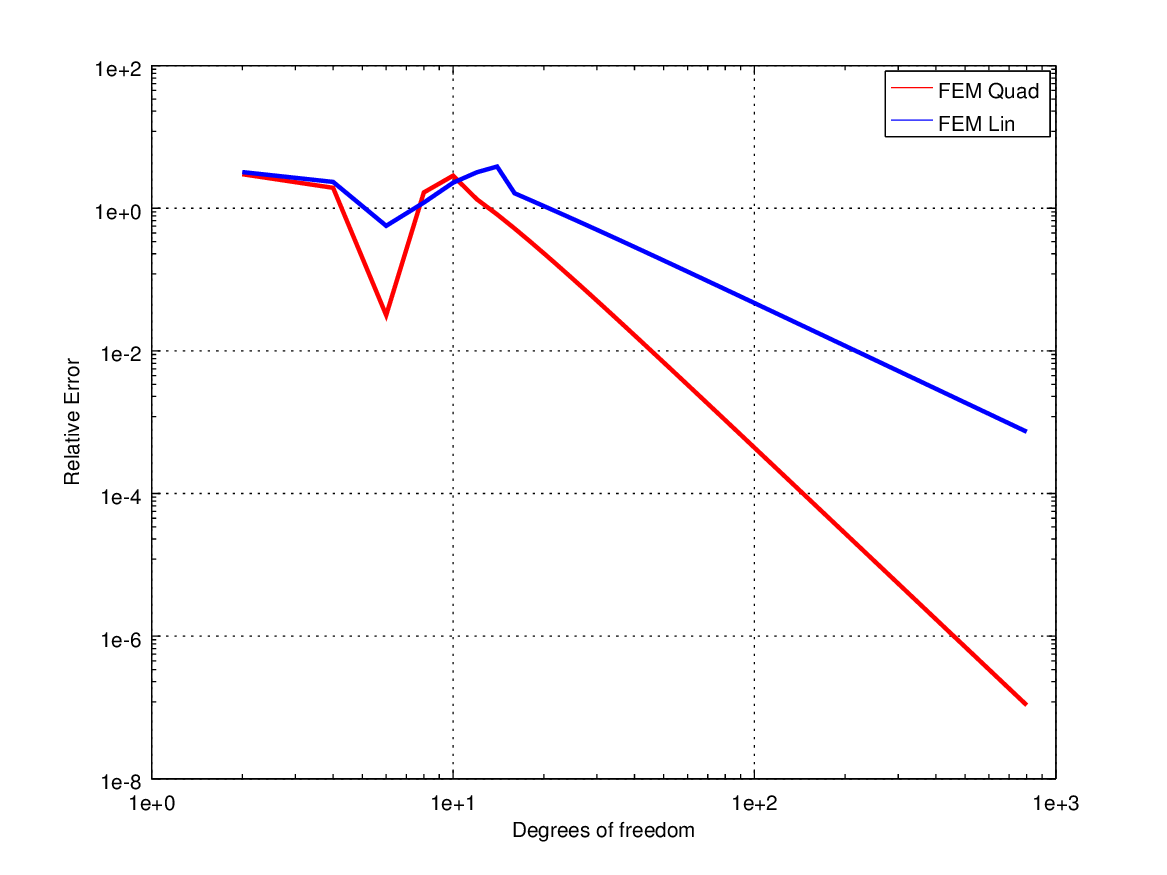
\includegraphics[width=0.6\textwidth]{../report/part1/figs/FEM/simuls_1D/convergence.png}

        \footnotesize{Erreur relative en fonction du nombre de degrés de libertés\\
        pour des éléments \textcolor{blue}{linéaires} et \textcolor{red}{quadratiques}}
		\end{center}
	\end{block}
\end{frame}

\begin{frame}
	\frametitle{Méthode de Galerkin Discontinue avec ondes planes}

	$$\int_\Omega \vec{v}^T\left(j\omega + A\nabla\right)\vec{u}\mathrm{d}\Gamma = 0$$

	\begin{block}{Généralités}
		\begin{itemize}
			\item Basée sur la formulation variationnelle de l'équation d'Helmholtz
            \item Utilisation des caractéristiques de l'EDP comme champ de test (Gabard \& Dazel, 2015, \textit{Int. J.
                Numer. Engng.})
			\item Possibilité d'utiliser de grands éléments
		\end{itemize}
	\end{block}

	\pause

	\begin{block}{Limites}
		\begin{itemize}
			\item Quasi-insensible aux petits détails
			\item Incompatibles avec (ou mal adaptés à) certains problèmes
		\end{itemize}
	\end{block}
\end{frame}

\begin{frame}[fragile]
	\frametitle{Méthode de Galerkin Discontinue avec ondes planes}
    \begin{wrapfigure}{r}{0.6\textwidth}
        \vspace{-0.1\textwidth}
        \begin{tikzpicture}[>=stealth,scale=0.4,transform shape]
        \begin{tikzpicture}[>=stealth]

	% waveguide
	\draw[thick] (0,.3) -- (0,.5) -- (7,.5) -- (7,2) -- (0,2) -- (0,2.2);
	\foreach \i in {0,...,5}{
		\draw[thick] (7,\i*0.3+0.5) -- ++(.3,.2);
	}
	
	% x axis
	\draw[->] (-.7,0) -- (8,0) node[right] {$x$};
	\draw (0,.1) -- ++(0,-.2) node[below] {$0$};
	\draw (7,.1) -- ++(0,-.2) node[below] {$L$};

	% waves
	% R
	\draw[<-] (-2.5,1) -- ++(1.5,0);
	\draw (-2,1.15) -- ++(0,-.3);
	\draw (-1.9,1.15) -- ++(0,-.3) node[below] {$R$};

	% I
	\draw[->] (-2.5,1.5) -- ++(1.5,0);
	\draw (-2,1.65) -- ++(0,-.3);
	\draw (-1.9,1.65) node[above] {$I$} -- ++(0,-.3);

\end{tikzpicture}


        \end{tikzpicture}
        \vspace{-0.2\textwidth}
    \end{wrapfigure}

	\begin{block}{Solution exacte en 1D...}
		\begin{center}
		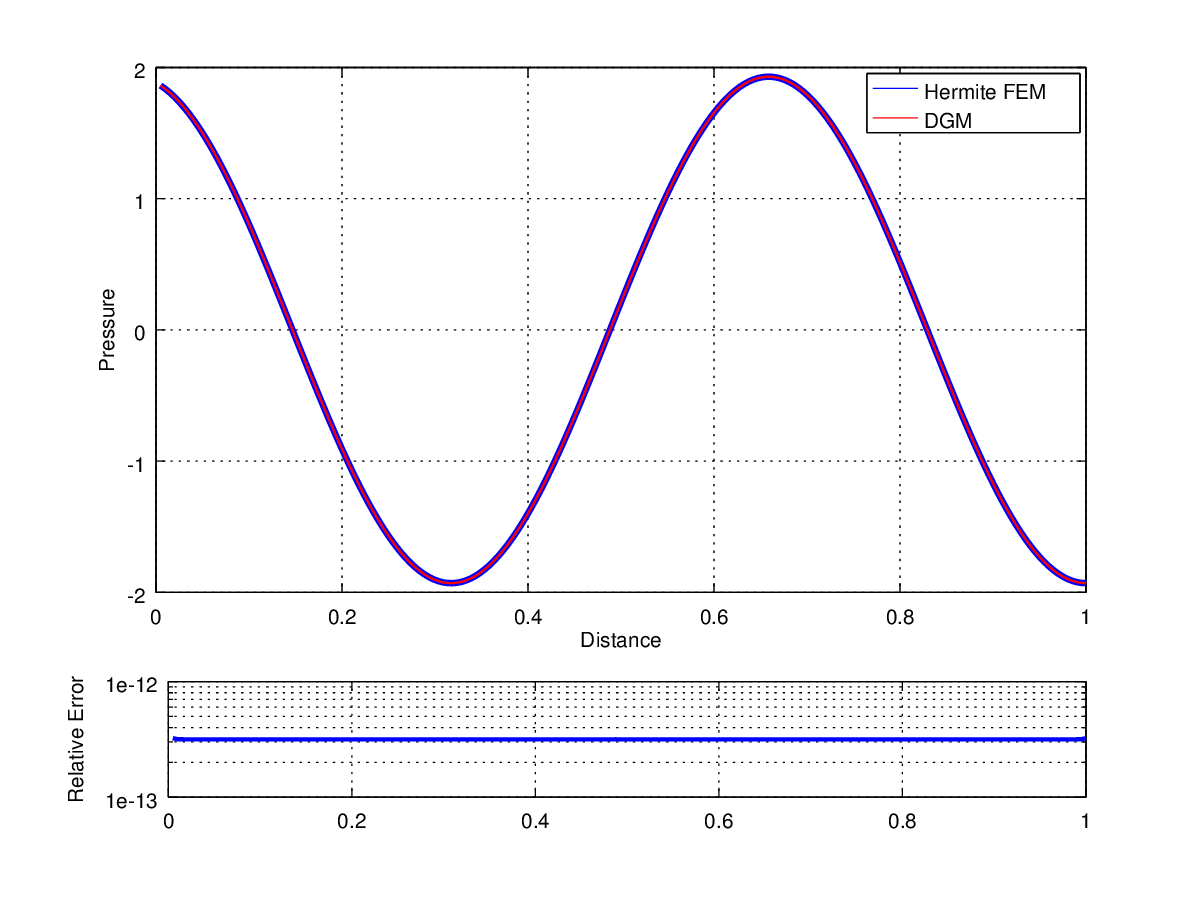
\includegraphics[width=0.6\textwidth]{comp_hermiteFEM_dgm.png}

        \footnotesize{Pression acoustique dans la cavité de \textcolor{blue}{référence} et calculée\\
        par \textcolor{red}{DGM} en fonction de la distance.}
		\end{center}
	\end{block}
\end{frame}

\section{Couplage}

\begin{frame}
	\frametitle{Conditions limites et FEM}

	\begin{block}{Classiquement}
		\begin{itemize}
			\item $R$ comme une inconnue
			\item Vecteurs et matrices étendues
			\item Traduction exacte des équations de continuité
		\end{itemize}

		\pause

		\begin{equation*}
			\left(~
			\begin{array}{cccc|c}
				&&&&-jk\\
				&&&&0\\
				& & \uul{K} - k^2\uul{M} & &\vdots \\
				&&&&0\\\hline
					1 & 0 & \cdots & 0& -1 \\
			\end{array}
			~\right)
			\left\{~
			\begin{matrix}
				\\
				\\
				\GP\\
				\\\hline
				R
			\end{matrix}
			~\right\} = 
			\left\{~
			\begin{matrix}
				-jk\\
				0\\
				\vdots\\
				0\\\hline
				1
			\end{matrix}
			~\right\}
		\end{equation*}
	\end{block}
\end{frame}

\begin{frame}
	\frametitle{Conditions limites et FEM}

	\begin{block}{Caractéristiquement...}
		\begin{itemize}
			\item Utilisation des caractéristiques pour exprimer la condition limite en $x=0$
			\item Besoin des fonctions de forme pour exprimer les champs
			\item Nécessité de dériver les fonctions de forme...
		\end{itemize}

		\pause

		\begin{equation*}
			\nabla p\bigg|_0 = - jk -\frac{jk}{2}\left[\left(\phi_1(0) + \frac{\phi'_1(0)}{jk}\right)\GP_1 + \left(\phi_2(0) + \frac{\phi'_2(0)}{jk}\right)\GP_2 \right]
		\end{equation*}
	\end{block}

	\begin{center}
		\alert{\textbf{Dérivation des fonctions de forme : \\perte d'un ordre de convergence ?}}
	\end{center}
\end{frame}

\begin{frame}
	\frametitle{Conditions limites et FEM}
	\begin{block}{Malheureusement... oui.}
		\begin{columns}[onlytextwidth]
            \begin{column}{0.6\textwidth}
                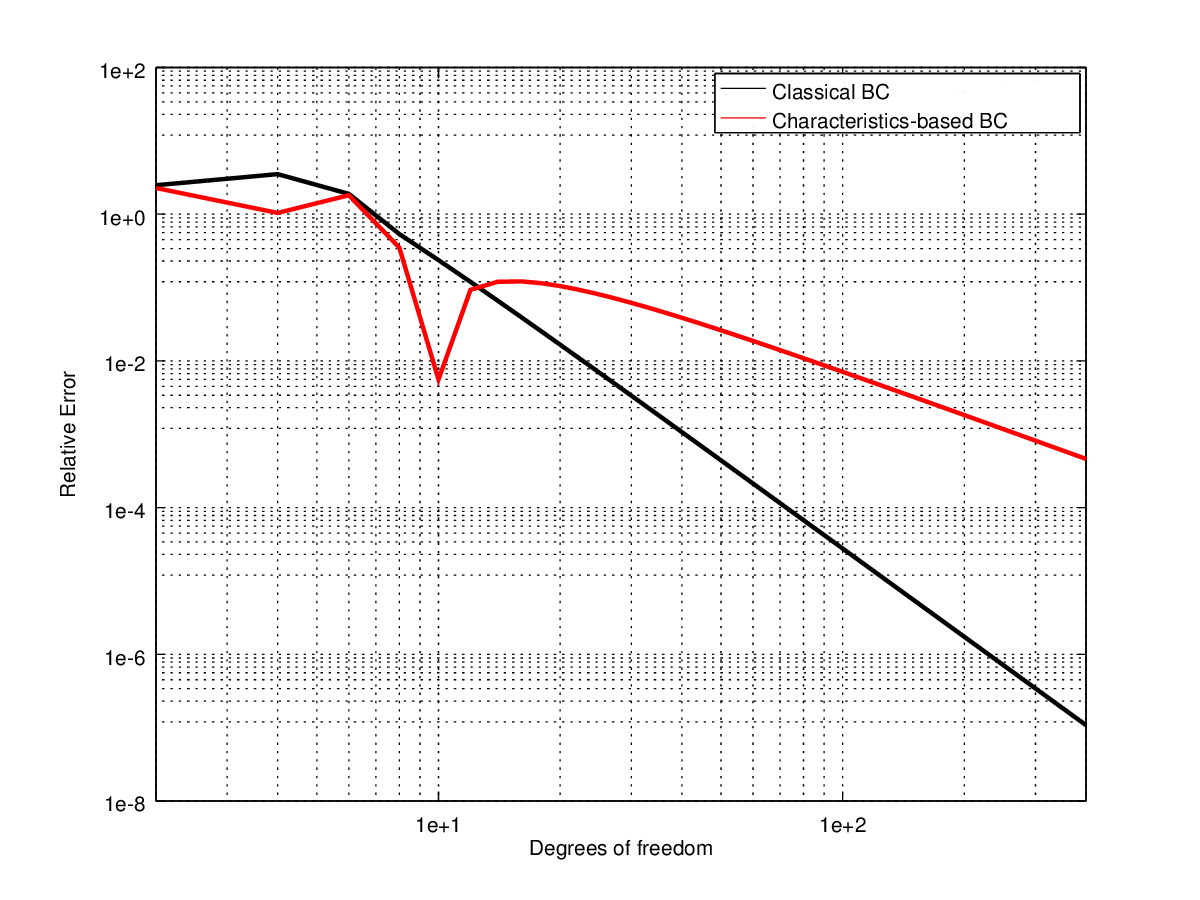
\includegraphics[width=\textwidth]{../report/part3/figs/convergence.png}
            \end{column}
            \begin{column}{0.4\textwidth}
            \footnotesize{Erreur relative en fonction du nombre d'éléments\\
            pour la méthode classique et pour des \textcolor{red}{caractéristiques}}
            \end{column}
		\end{columns}
	\end{block}

	\pause

	\begin{center}
		\alert{\textbf{
		Comment éviter ce (gros) désagrément ?
		}}
	\end{center}
\end{frame}


\section{Amélioration de la convergence}

\begin{frame}
	\frametitle{Dérivation «naturelle» ?}

	\textbf{Question :} Existe-t-il une méthode d'interpolation donnant \alert{directement accès} à la dérivée du champ
	?

	\pause
	\bigskip

	\textbf{Réponse :} Oui ! L'interpolation par \alert{splines d'Hermite} !

	\begin{equation*}
		p_e(x) = \left[\H{00}(x)\big|\H{10}(x)\big|\H{01}(x)\big|\H{11}(x)\right]\begin{Bmatrix}p_1\\p'_1\\p_2\\p'_2\end{Bmatrix}
	\end{equation*}
\end{frame}

\begin{frame}
	\frametitle{Convergence}
	\begin{block}{Words are good... show me the curve !}
		\begin{columns}[onlytextwidth]
		\begin{column}{0.6\textwidth}
			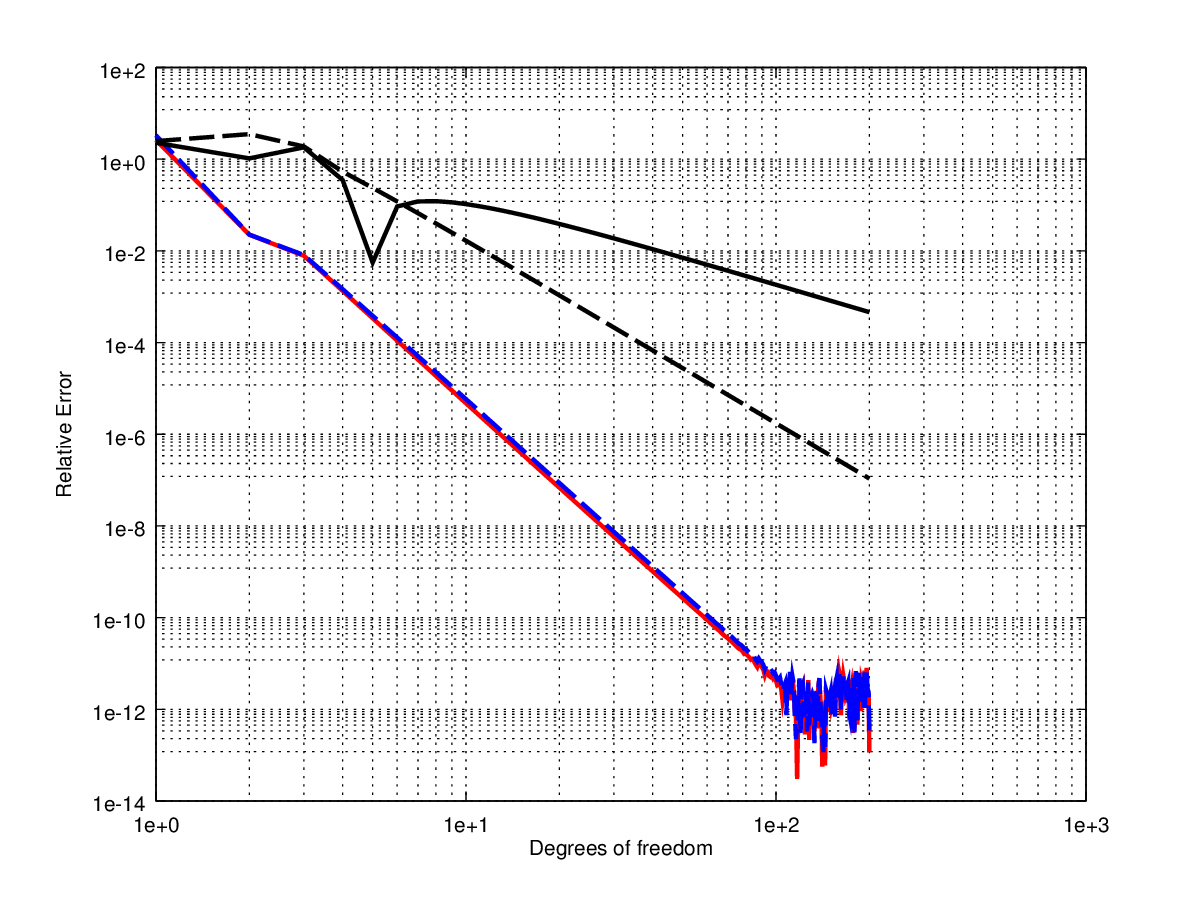
\includegraphics[width=\textwidth]{../report/part4/figs/herm_comp.png}
		\end{column}
		\begin{column}{0.4\textwidth}
            \footnotesize{Erreur relative en fonction du nombre de degrés de liberté pour les méthodes classique
            (-~-) et des caractéristiques (---) pour des éléments quadratiques et des \textcolor{blue}{spline}
            \textcolor{red}{d'Hermite}}
		\end{column}
		\end{columns}
	\end{block}

    \pause

    \begin{center}
        \alert{Ça converge !}

        \pause

        Mieux que les éléments quadratiques...\pause pour les deux méthodes
    \end{center}
\end{frame}

\section{Et ensuite ?}

\begin{frame}
	\frametitle{Pistes pour la suite}

	\begin{itemize}
		\item Coupler plusieurs éléments DGM et FEM ensemble
		\item Analyser le comportement du couplage en 2D
		\item Appliquer la méthode à de vrais problèmes
		\item Analyser l'évolution du temps de calcul
		\item Auto-sélection de la méthode la plus adaptés à certains groupes d'éléments sur un maillage quelconque
		\item etc...
	\end{itemize}
\end{frame}

\section*{Conclusion}

\begin{frame}
	\frametitle{Conclusion}
	\begin{itemize}
		\item Prise en main et analyse de 2 méthodes de calcul
		\item Introduction aux possibilités de couplage ente méthodes
		\item Travail sur un sujet de recherche intéressant
		\item Possibilités de poursuite du projet
	\end{itemize}
\end{frame}

\begin{frame}
    \frametitle{References}

    \begin{itemize}
        \item  G. Gabard, O.  Dazel, \textbf{A discontinuous Galerkin Method with Plane Waves for Sound Absorbing
            Materials}, 2015, \textit{Int. J.  Numer. Engng}, à paraître
        \item  G. Gabard, P. Gamallo, T. Huttunen, \textbf{A comparison of wave-based discontinuous Galerkin, ultra-week
            and least-square method for wave problems}, 2011, \textit{Int. J.  Numer. Engng}, vol. 85 no 3
        \item \textbf{Analyse Numérique : une approche mathématique}, M. Schatzman
    \end{itemize}
\end{frame}

\plain{Merci !\\
\vspace{0.25\textwidth}
Des questions ?\\
\vspace{0.15\textwidth}
\scriptsize{\texttt{mathieu@matael.org}}
}

\end{document}
